\documentclass[conference]{IEEEtran}
\IEEEoverridecommandlockouts
\usepackage[utf8]{inputenc}
\usepackage[T1]{fontenc}
\usepackage[brazil]{babel}
\usepackage{cite}
\usepackage{amsmath,amssymb,amsfonts}
\usepackage{algorithmic}
\usepackage{algorithm}
\usepackage{graphicx}
\usepackage{textcomp}
\usepackage{xcolor}
\usepackage{booktabs}

% Numeric results generated automatically from experiments/pco213/santander
% by scripts/pco213_make_article_macros.py — do not edit by hand.
% Auto-generated by scripts/pco213_make_article_macros.py — do not edit.
\newcommand{\DesignRuns}{21}
\newcommand{\ValPoints}{25}
\newcommand{\PooledRtwoAUC}{0{,}963}
\newcommand{\PooledRtwoLL}{0{,}995}
\newcommand{\CondNumber}{11{,}8}
\newcommand{\RelRmseAUC}{46{,}1\%}
\newcommand{\RelRmseLL}{4{,}3\%}
\newcommand{\GapMetaDirect}{0{,}00347}
\newcommand{\NBWeightAUC}{0{,}62}
\newcommand{\NBWeightLL}{0{,}77}
\newcommand{\TotalWallMin}{9{,}9}
\newcommand{\MaxUnivarAUC}{0{,}567}
\newcommand{\MedUnivarAUC}{0{,}524}
\newcommand{\MaxAbsCorr}{0{,}021}
\newcommand{\BaseModelsSummary}{O melhor modelo individual em OOF foi o Gaussian NB (AUC média 0{,}888), seguido de perto pelo XGBoost (0{,}882); o $k$-NN ficou substancialmente abaixo (0{,}726), como esperado em 200 dimensões.}
\newcommand{\HoldoutSummary}{Em perda logarítmica no holdout, as misturas otimizadas (direta: 0{,}2115; Scheffé: 0{,}2154) superaram o melhor modelo individual (0{,}2170), o stacking (0{,}2171) e, com folga, o voto uniforme (0{,}2271). Em ROC-AUC as diferenças são pequenas: a melhor mistura (0{,}8908, varredura direta) e o voto uniforme (0{,}8896) praticamente empatam, ambos acima do melhor modelo individual (0{,}8822).}
\newcommand{\StatsSummary}{em perda logarítmica, a mistura de Scheffé foi significativamente melhor ($t=35{,}0$; p<0{,}001) que o voto uniforme e significativamente melhor ($t=6{,}3$; p<0{,}001) que o stacking; em ROC-AUC, foi estatisticamente indistinguível (p=0{,}813) do voto uniforme e significativamente melhor ($t=11{,}7$; p<0{,}001) que o melhor modelo individual — coerente com uma região quase ótima ampla que contém o centroide do simplex.}
\newcommand{\CoefReading}{O termo cruzado de maior magnitude foi gnb--knn ($\beta=0{,}305$), identificando o par de famílias com maior complementaridade sob AUC.}


\def\BibTeX{{\rm B\kern-.05em{\sc i\kern-.025em b}\kern-.08em
    T\kern-.1667em\lower.7ex\hbox{E}\kern-.125emX}}
\begin{document}

\title{Otimização de Ensembles de Classificadores por Arranjo de Misturas e Metamodelagem de Superfície de Resposta}

\author{\IEEEauthorblockN{Caio Tertuliano Ribeiro}
\IEEEauthorblockA{\textit{Instituto de Engenharia de Sistemas e Tecnologia da Informação} \\
\textit{Universidade Federal de Itajubá (UNIFEI)}\\
Itajubá, Brasil \\
Matrícula 2026102152 --- caio.tertu99@gmail.com}
}

\maketitle

\begin{abstract}
A combinação ponderada de classificadores heterogêneos é uma das técnicas mais eficazes em problemas tabulares, mas os pesos do ensemble são usualmente escolhidos por busca ad hoc, sem caracterização estatística. Neste trabalho, os pesos de um ensemble de cinco classificadores são tratados como componentes de uma mistura: restritos ao simplex, são planejados por um arranjo de misturas, avaliados sem vazamento sobre predições out-of-fold e modelados por um polinômio canônico de Scheffé, que decompõe o desempenho em contribuições individuais e complementaridades entre pares de modelos. O estudo usa o conjunto de dados real da competição Santander Customer Transaction Prediction (200 mil observações, 200 variáveis, 10\% de positivos). O metamodelo quadrático reproduziu a superfície de perda logarítmica com erro externo de \RelRmseLL\ da amplitude observada, e seu ótimo concordou com o ótimo global obtido por otimização direta nos componentes dominantes. No conjunto de teste, a mistura otimizada superou o melhor modelo individual, o stacking logístico e o voto uniforme em perda logarítmica; em ROC-AUC mostrou-se estatisticamente indistinguível do voto uniforme, e o próprio metamodelo explica o porquê: a região quase ótima da superfície é ampla e contém o centroide do simplex. Os coeficientes do metamodelo forneceram uma leitura interpretável da estrutura de complementaridade entre as famílias de modelos, dominada pelo par Naive Bayes e XGBoost.
\end{abstract}

\begin{IEEEkeywords}
ensembles, arranjo de misturas, superfície de resposta, polinômio de Scheffé, validação cruzada, classificação binária
\end{IEEEkeywords}

\section{Introdução}
Métodos de \emph{ensemble} combinam as predições de múltiplos classificadores e figuram entre as técnicas de melhor desempenho em dados tabulares \cite{b1}. Na forma mais simples e amplamente utilizada — o voto suave ponderado — a probabilidade final é uma combinação convexa das probabilidades previstas pelos modelos-base. Surge então uma pergunta prática: \emph{como escolher os pesos dessa combinação de maneira fundamentada, e o que a estrutura da superfície de desempenho revela sobre os modelos combinados?}

Na prática corrente, os pesos são definidos por heurísticas (pesos uniformes), por busca gulosa \cite{b4} ou por um meta-modelo de \emph{stacking} \cite{b2}, abordagens que produzem um vetor de pesos, mas não uma \emph{caracterização} da superfície de desempenho. A observação central deste trabalho é geométrica: pesos não negativos que somam um vivem exatamente no domínio canônico dos \emph{experimentos com misturas} \cite{b6,b7}. Isso permite transpor um ferramental estatístico maduro — arranjos simplex-lattice, polinômios de Scheffé, validação de metamodelos — para a análise de ensembles: cada classificador é um ``ingrediente'', o vértice puro do simplex corresponde a usar um único modelo, e o centroide é o voto uniforme.

É importante declarar, desde já, uma questão de honestidade computacional: sobre predições \emph{out-of-fold} (OOF) pré-computadas, avaliar qualquer vetor de pesos custa um produto matriz-vetor, e a perda logarítmica é convexa nos pesos — o ótimo global pode ser obtido diretamente por programação sequencial quadrática (SLSQP) em milissegundos. O metamodelo de misturas \emph{não} se justifica, portanto, como atalho computacional. A contribuição proposta é inferencial e interpretativa: os coeficientes lineares do polinômio de Scheffé estimam a contribuição de cada classificador, os coeficientes cruzados quantificam a \emph{complementaridade} entre pares de modelos — conectando-se à decomposição de ambiguidade de ensembles \cite{b5} — e a superfície ajustada delimita regiões quase ótimas de pesos. A otimização direta é usada como \emph{validador} do metamodelo.

O objetivo principal é verificar, em um conjunto de dados real de competição (Santander Customer Transaction Prediction \cite{b13}), se o ensemble com pesos otimizados por essa metodologia supera \emph{baselines} internos honestos (melhor modelo individual, voto uniforme, stacking logístico) sob um protocolo estrito contra vazamento de dados. Os objetivos secundários são: (i) quantificar a adequação do metamodelo de Scheffé por validação externa; (ii) interpretar os coeficientes de complementaridade entre cinco famílias de modelos; e (iii) analisar a divergência entre os pesos ótimos sob métrica de ordenação (ROC-AUC) e sob métrica de calibração (perda logarítmica).

\section{Trabalhos Relacionados}
A literatura de combinação de classificadores é extensa. Dietterich \cite{b1} sistematiza as razões pelas quais ensembles funcionam (estatística, computacional e representacional), enquanto Krogh e Vedelsby \cite{b5} demonstram que o erro do ensemble se decompõe em erro médio dos componentes menos a \emph{ambiguidade} (diversidade) entre eles — resultado que fundamenta a interpretação dos termos cruzados do metamodelo aqui proposto.

Wolpert \cite{b2} introduziu o \emph{stacked generalization}, em que um meta-modelo é ajustado sobre predições out-of-fold; Breiman \cite{b3} propôs a versão regularizada com pesos não negativos, observando que a restrição ao simplex melhora a generalização — precisamente o domínio explorado neste trabalho, porém sem o desenho experimental nem a leitura de superfície. Caruana \emph{et al.} \cite{b4} popularizaram a seleção gulosa de ensembles a partir de bibliotecas de modelos, método eficaz, mas que não produz inferência sobre a estrutura de complementaridade. Do lado do planejamento de experimentos, Scheffé \cite{b6} e Cornell \cite{b7} estabeleceram os arranjos simplex-lattice e os polinômios canônicos para misturas, aplicados tradicionalmente à formulação de produtos químicos e alimentos.

A lacuna identificada é a ausência de estudos que tratem os pesos de um ensemble como problema formal de \emph{mistura estatística}, com arranjo experimental no simplex, metamodelo canônico e validação externa — combinando a tradição de DOE/RSM com a prática de ensembles. Este trabalho preenche essa lacuna em um estudo de caso controlado e reprodutível, usando classificadores clássicos consolidados \cite{b8,b9} e o protocolo de inferência corrigida para validação cruzada repetida de Nadeau e Bengio \cite{b10,b11}.

\section{Metodologia}
A Fig.~\ref{fig:fluxo} apresenta o diagrama geral da proposta; as subseções detalham cada etapa. Toda a implementação foi realizada em Python com scikit-learn \cite{b12} e XGBoost \cite{b8}.

\begin{figure}[htbp]
\centerline{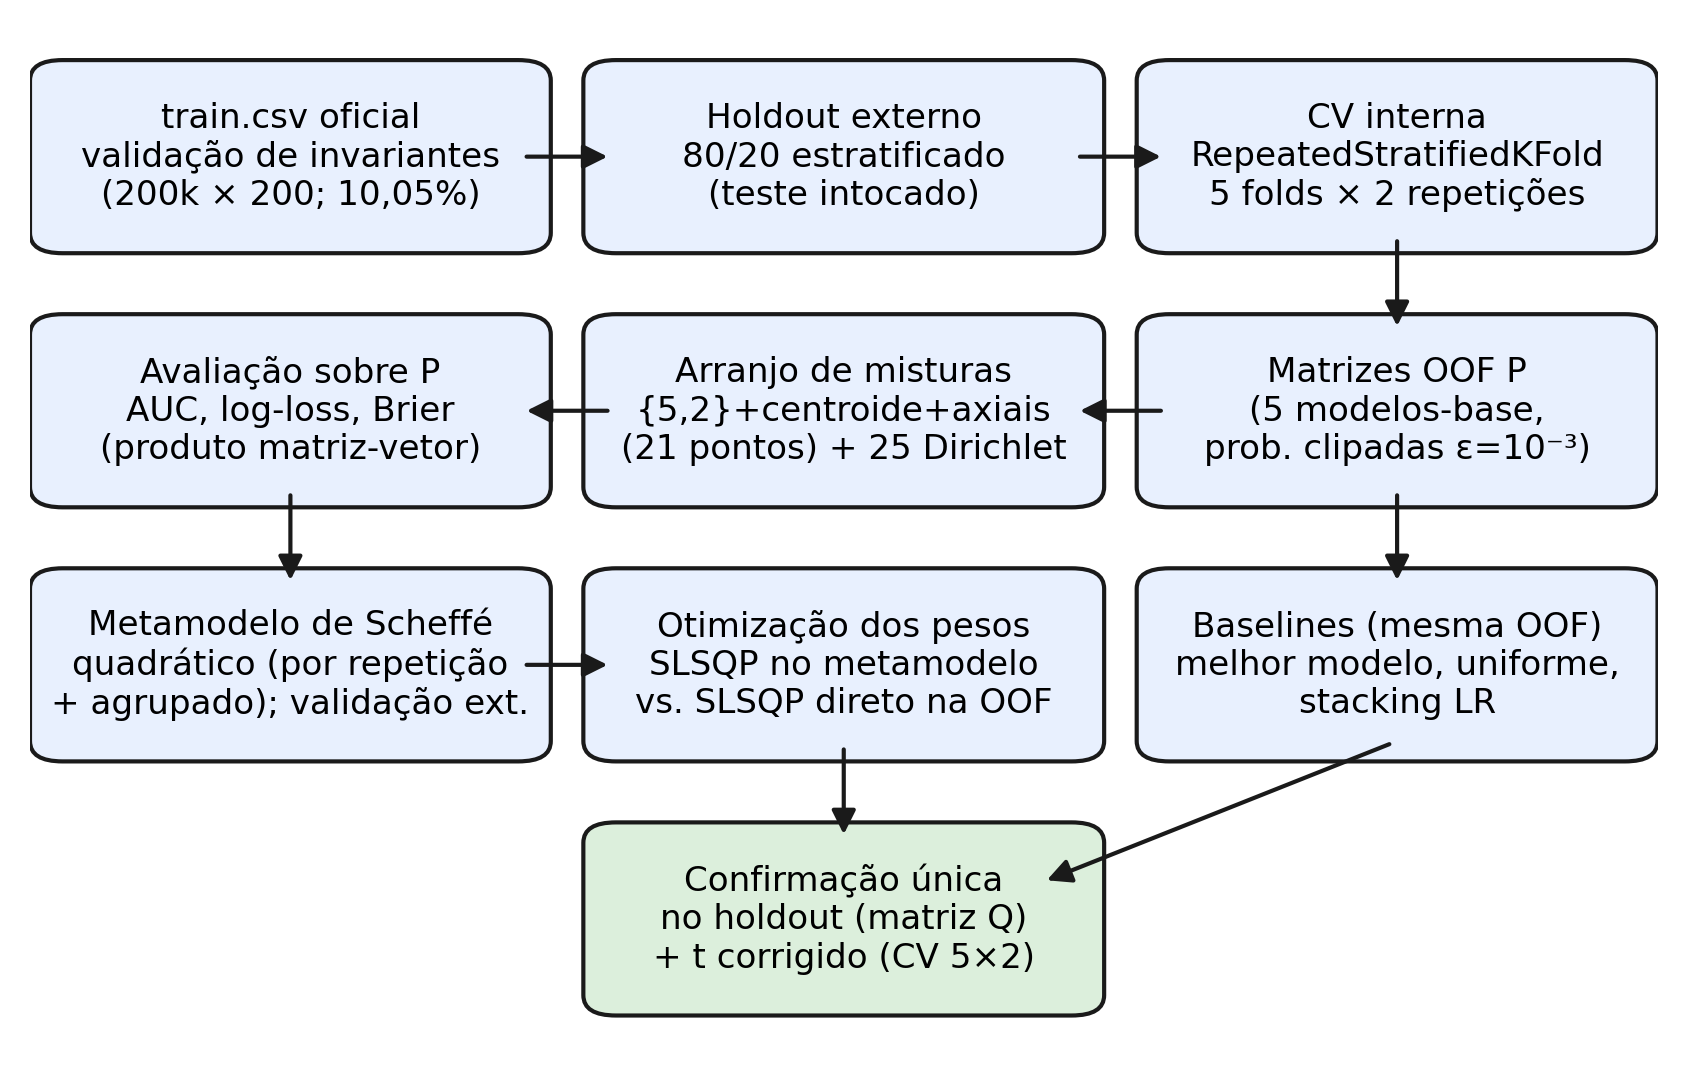
\includegraphics[width=\columnwidth]{Figures/fig1_metodologia.png}}
\caption{Diagrama geral da metodologia proposta: da validação do dado bruto à confirmação única no conjunto de teste.}
\label{fig:fluxo}
\end{figure}

\subsection{Formulação do problema}
Sejam $M$ classificadores-base e $p_j(x)\in[0,1]$ a probabilidade prevista pelo modelo $j$ para a classe positiva. O ensemble ponderado é definido por
\begin{equation}
p_{\mathrm{ens}}(x;\,w)=\sum_{j=1}^{M} w_j\, p_j(x),
\qquad w\in\Delta^{M-1},
\label{eq:ens}
\end{equation}
onde $\Delta^{M-1}=\{w\in\mathbb{R}^M : w_j\ge 0,\ \sum_j w_j=1\}$ é o simplex. Os vértices de $\Delta^{M-1}$ reproduzem os modelos individuais e o centroide $w_j=1/M$ é o voto uniforme.

O desempenho do ensemble como função dos pesos, $\eta(w)$, é modelado pelo polinômio canônico quadrático de Scheffé \cite{b6,b7}, sem intercepto e sem termos quadráticos puros (consequência da restrição de soma unitária):
\begin{equation}
\eta(w)=\sum_{j=1}^{M}\beta_j w_j+\sum_{j<l}\beta_{jl}\, w_j w_l .
\label{eq:scheffe}
\end{equation}
O coeficiente $\beta_j$ estima a resposta no vértice $j$ (o desempenho do modelo puro); $\beta_{jl}$ mede o desvio da mistura binária em relação à interpolação linear dos desempenhos — a \emph{complementaridade} entre os modelos $j$ e $l$. Para perdas convexas nos pesos (perda logarítmica e Brier), a desigualdade de Jensen garante que a mistura nunca é pior que a interpolação linear; nessas métricas o sinal favorável de $\beta_{jl}$ é estrutural, e a pergunta científica passa a ser a \emph{magnitude relativa} das complementaridades. Em ROC-AUC, não convexa em $w$, o sinal é livre. O escore de Brier, exatamente quadrático em $w$, é reproduzido de forma exata pelo metamodelo \eqref{eq:scheffe} e é usado como teste de sanidade do pipeline, não como evidência de adequação.

A busca pelos pesos ótimos é formulada como
\begin{equation}
w^{\ast}=\arg\min_{w\in\Delta^{M-1}} \mathcal{L}\!\left(y,\;P\,w\right),
\label{eq:opt}
\end{equation}
onde $P\in\mathbb{R}^{n\times M}$ é a matriz de probabilidades OOF e $\mathcal{L}$ a perda logarítmica. Como \eqref{eq:opt} é convexo, sua solução por SLSQP multi-partida é o ótimo global e serve de referência para validar o ótimo do metamodelo.

\subsection{Arranjo de misturas e metamodelagem}
O arranjo experimental combina o simplex-lattice $\{5,2\}$ (5 vértices e 10 pontos médios de aresta), o centroide global e 5 pontos axiais interiores ($w_j=(M{+}1)/2M$ no componente axial), totalizando \DesignRuns\ corridas — suporte suficiente para os 15 termos de \eqref{eq:scheffe} com 6 graus de liberdade residuais no ajuste por repetição e 27 no ajuste agrupado. Cada ponto do arranjo é avaliado sobre as matrizes OOF (Seção~\ref{sec:protocolo}) em ROC-AUC, perda logarítmica e Brier. O metamodelo é ajustado por mínimos quadrados ordinários sem eliminação de termos (a interpretação canônica exige o conjunto completo \cite{b7}), separadamente por repetição da validação cruzada — produzindo faixas de estabilidade dos coeficientes sob repartição — e no conjunto agrupado das duas repetições. A adequação é verificada por \emph{validação externa}: \ValPoints\ pontos adicionais amostrados uniformemente no simplex (distribuição de Dirichlet), não utilizados no ajuste, nos quais se reporta o erro quadrático médio (RMSE) absoluto e relativo à amplitude da resposta.

\subsection{Protocolo experimental contra vazamento}
\label{sec:protocolo}
O protocolo, pré-registrado no repositório do projeto, é resumido no Algoritmo~\ref{alg:pipeline}:
(i) o conjunto rotulado oficial é validado contra invariantes (número de linhas, colunas, taxa de positivos, ausência de faltantes) e o conjunto de teste da competição, sem rótulos, é descartado;
(ii) separa-se um \emph{holdout} externo estratificado de 20\%, intocado até a confirmação final;
(iii) no treino, executa-se validação cruzada estratificada repetida (5 \emph{folds} $\times$ 2 repetições = 10 rodadas); cada modelo-base é ajustado uma vez por \emph{fold}, com todas as transformações dependentes de dados (padronização) ajustadas dentro do \emph{fold}, gerando matrizes OOF $P$;
(iv) as probabilidades dos \emph{componentes} são recortadas ao intervalo $[\varepsilon,1-\varepsilon]$, $\varepsilon=10^{-3}$, antes da perda logarítmica (kNN e Naive Bayes produzem probabilidades exatamente 0/1), preservando a linearidade de \eqref{eq:ens} nos pesos;
(v) toda seleção — pesos, limiar de decisão, meta-modelo de stacking — usa exclusivamente as matrizes OOF;
(vi) os cinco modelos são reajustados uma única vez no treino completo e a comparação final é feita uma única vez no holdout.
O limiar de F1 e acurácia balanceada é escolhido, para cada método, sobre suas próprias predições OOF e aplicado sem reajuste ao holdout. Para as comparações formais entre métodos utiliza-se o teste $t$ corrigido para validação cruzada repetida \cite{b10,b11} sobre as $J=10$ diferenças por \emph{fold},
\begin{equation}
t=\bar{d}\Big/\sqrt{s_d^{2}\left(\tfrac{1}{J}+\rho\right)},\qquad \rho=\tfrac{n_{\mathrm{te}}}{n_{\mathrm{tr}}}=0{,}25,
\label{eq:nb}
\end{equation}
reportado com a ressalva de que, com um único conjunto de dados, o teste permanece aproximado.

\begin{algorithm}[htbp]
\caption{Pipeline do estudo (pseudocódigo)}
\label{alg:pipeline}
\begin{algorithmic}[1]
\STATE valida invariantes do dado bruto; remove identificador
\STATE $(\mathcal{D}_{\mathrm{tr}},\mathcal{D}_{\mathrm{te}})\leftarrow$ split estratificado 80/20
\FOR{repetição $r=1,2$}
  \FOR{\emph{fold} $k=1,\dots,5$}
    \STATE ajusta os $M$ modelos em $\mathcal{D}_{\mathrm{tr}}\setminus f_k$; prediz $f_k$
  \ENDFOR
  \STATE monta $P^{(r)}$ (OOF) com probabilidades recortadas
\ENDFOR
\STATE gera arranjo $W$ (\DesignRuns\ pontos) e validação $W_{\mathrm{val}}$ (\ValPoints)
\STATE avalia $W, W_{\mathrm{val}}$ sobre $P^{(r)}$ (AUC, log-loss, Brier)
\STATE ajusta Scheffé \eqref{eq:scheffe} por repetição e agrupado
\STATE $w^{\ast}_{\mathrm{meta}}\leftarrow$ ótimo de \eqref{eq:scheffe}; $w^{\ast}_{\mathrm{SLSQP}}\leftarrow$ ótimo de \eqref{eq:opt}
\STATE compara com \emph{baselines} na OOF; escolhe limiares na OOF
\STATE reajusta modelos no treino completo; confirma tudo em $\mathcal{D}_{\mathrm{te}}$
\end{algorithmic}
\end{algorithm}

\subsection{Modelos-base e \emph{baselines}}
O zoológico tem $M=5$ famílias deliberadamente heterogêneas, com configurações leves e fixas (sem busca de hiperparâmetros, decisão pré-registrada de escopo): regressão logística (com padronização), Gaussian Naive Bayes, $k$-NN ($k=100$, busca exata, com padronização), Random Forest \cite{b9} (200 árvores, folha mínima 20) e XGBoost \cite{b8} (histograma, 400 árvores, profundidade 6). Evitou-se um segundo \emph{gradient boosting}: componentes quase colineares tornam os coeficientes de \eqref{eq:scheffe} não identificáveis. Os \emph{baselines} são: melhor modelo individual (selecionado na OOF), voto uniforme (centroide do arranjo), \emph{stacking} com regressão logística ajustada sobre as mesmas matrizes OOF \cite{b2} e a otimização direta \eqref{eq:opt}. Um microbenchmark prévio (uma amostra pequena, um \emph{fold} por modelo) estimou o custo total e selecionou o modo de execução com dado completo, dentro do teto pré-registrado de 2 horas.

\section{Dados e Análise Exploratória}
O conjunto Santander Customer Transaction Prediction \cite{b13} contém 200.000 observações rotuladas, 200 variáveis numéricas anonimizadas (\texttt{var\_0}--\texttt{var\_199}) e alvo binário com 10,05\% de positivos; a métrica oficial da competição é ROC-AUC. A validação de invariantes confirmou a íntegra do arquivo (inclusive contra o tamanho oficial publicado) e a ausência de valores faltantes e de duplicatas; não há variáveis categóricas.

Sendo as variáveis anonimizadas, a análise exploratória é estrutural. As distribuições por classe mostram separação fraca e difusa: a maior ROC-AUC univariada é \MaxUnivarAUC\ (mediana \MedUnivarAUC), de modo que nenhum pequeno subconjunto de variáveis domina o problema. O achado central é a estrutura de correlação: a matriz de correlação amostral é praticamente a identidade (Fig.~\ref{fig:corr}), com $|r|$ máximo fora da diagonal de \MaxAbsCorr. Essa quase-independência explica um fato notório da competição — modelos ingênuos por variável, como o Naive Bayes, são competitivos com \emph{gradient boosting} \cite{b14} — e é exatamente o cenário em que famílias de modelos distintas erram em pontos diferentes, favorecendo misturas não triviais. Como consequências de pré-processamento: não há imputação nem codificação; a padronização é ajustada dentro de cada \emph{fold} apenas para os modelos sensíveis à escala; não se usa reamostragem (o desbalanceamento é tratado por estratificação e pela escolha de métricas); e as variáveis transdutivas de contagem usadas na competição (a ``mágica'') são proibidas por dependerem do conjunto de teste.

\begin{figure}[htbp]
\centerline{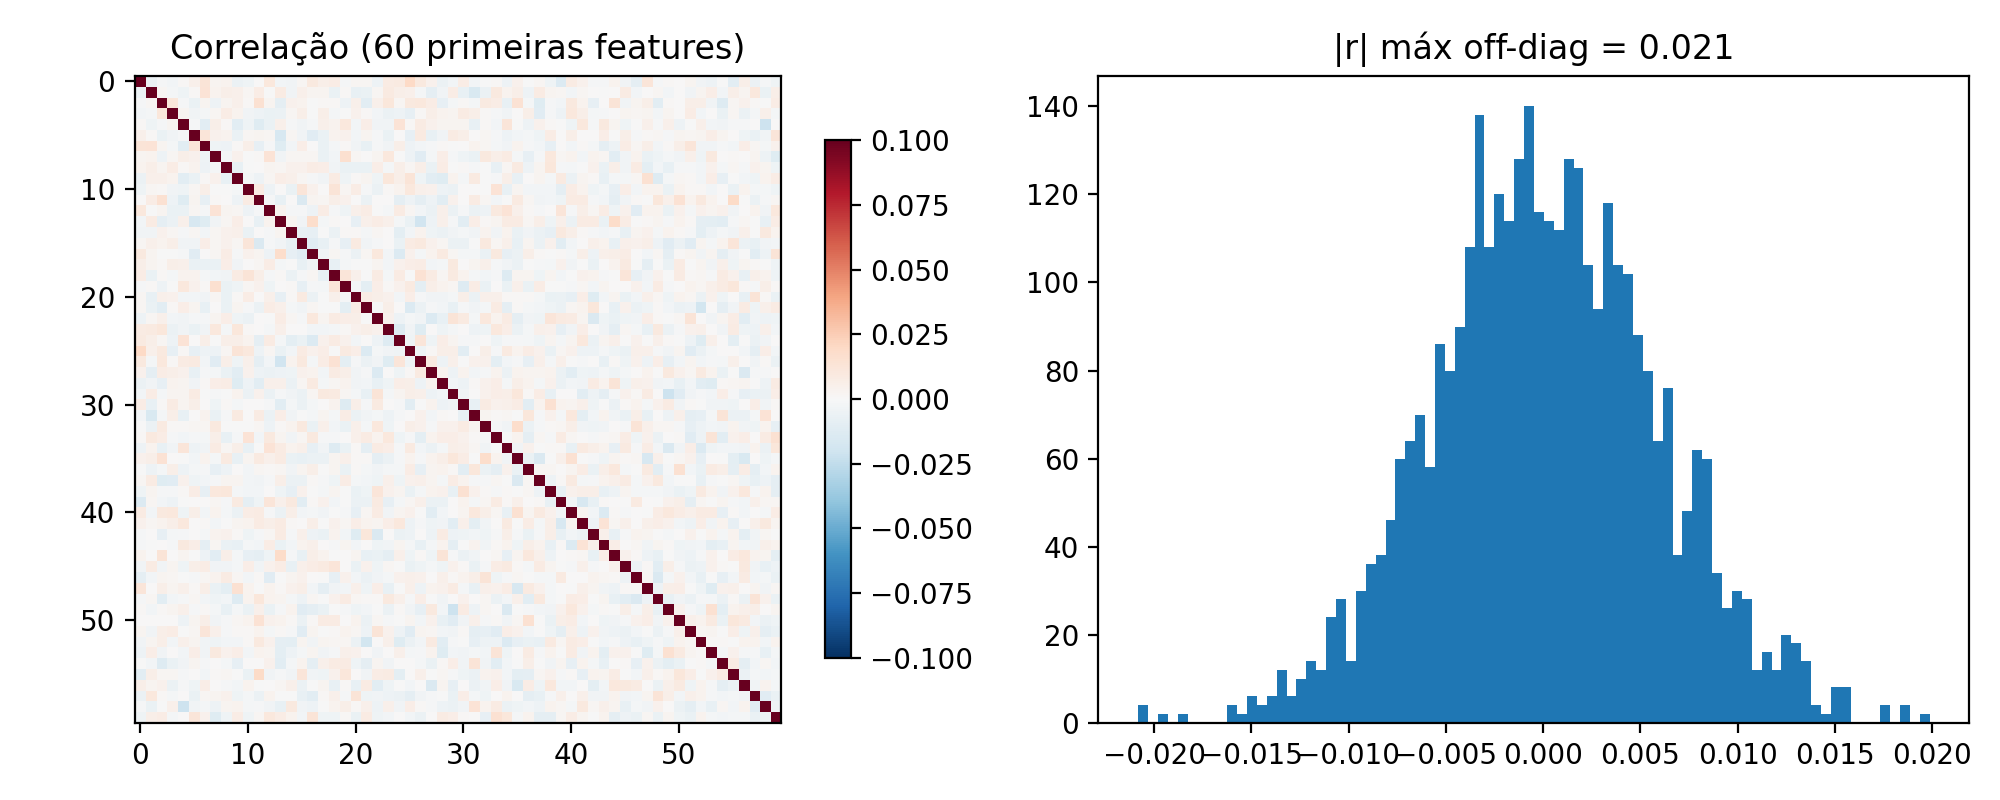
\includegraphics[width=\columnwidth]{Figures/fig2_eda_correlation.png}}
\caption{Estrutura de correlação (60 primeiras variáveis, amostra de 30 mil linhas): matriz praticamente identidade — quase-independência entre variáveis.}
\label{fig:corr}
\end{figure}

\section{Experimentos e Resultados}
\subsection{Modelos-base}
A Tabela~\ref{tab:base} resume o desempenho OOF dos cinco modelos nas 10 rodadas. \BaseModelsSummary\ A heterogeneidade é a matéria-prima da mistura: as correlações de erro entre famílias distintas ficaram bem abaixo do limiar de gêmeos pré-registrado.

\begin{table}[htbp]
\caption{Desempenho OOF dos modelos-base (média $\pm$ desvio entre 10 \emph{folds})}
\begin{center}
\small\setlength{\tabcolsep}{4pt}
\begin{tabular}{lccc}
\toprule
Modelo & ROC-AUC & log-loss & Brier \\
\midrule
Gaussian NB & 0{,}8879 $\pm$ 0{,}0038 & 0{,}2108 $\pm$ 0{,}0025 & 0{,}0604 $\pm$ 0{,}0006 \\
XGBoost & 0{,}8820 $\pm$ 0{,}0044 & 0{,}2194 $\pm$ 0{,}0027 & 0{,}0632 $\pm$ 0{,}0007 \\
Reg.\ Logística & 0{,}8592 $\pm$ 0{,}0043 & 0{,}2321 $\pm$ 0{,}0023 & 0{,}0665 $\pm$ 0{,}0006 \\
Random Forest & 0{,}8457 $\pm$ 0{,}0040 & 0{,}2748 $\pm$ 0{,}0006 & 0{,}0793 $\pm$ 0{,}0001 \\
$k$-NN & 0{,}7258 $\pm$ 0{,}0045 & 0{,}3527 $\pm$ 0{,}0012 & 0{,}0922 $\pm$ 0{,}0001 \\
\bottomrule
\end{tabular}
\label{tab:base}
\end{center}
\end{table}

\subsection{Metamodelo de Scheffé}
O metamodelo quadrático agrupado apresentou $R^2=\PooledRtwoLL$ para a perda logarítmica e $R^2=\PooledRtwoAUC$ para ROC-AUC, com número de condição \CondNumber\ da matriz canônica. A validação externa (\ValPoints\ pontos Dirichlet não usados no ajuste) revelou uma assimetria informativa: em perda logarítmica o metamodelo é excelente (RMSE de \RelRmseLL\ da amplitude; $R^2$ externo de 0,95), enquanto em AUC a superfície é tão achatada (amplitude total de apenas 0,016 no simplex) que o RMSE externo, embora pequeno em termos absolutos (0,008), corresponde a \RelRmseAUC\ da amplitude — limitação pré-registrada no protocolo: em superfícies quase planas, medidas relativas de adequação externa são mal condicionadas. Como previsto pela teoria, o Brier — exatamente quadrático nos pesos — foi reproduzido com $R^2=1$ e RMSE externo nulo, confirmando a sanidade numérica do pipeline. A Fig.~\ref{fig:ternary} mostra a superfície de AUC prevista na face dos três componentes dominantes, com os pontos do arranjo sobrepostos; a Fig.~\ref{fig:coef} apresenta os coeficientes com faixas de estabilidade entre repetições. \CoefReading

\begin{figure}[htbp]
\centerline{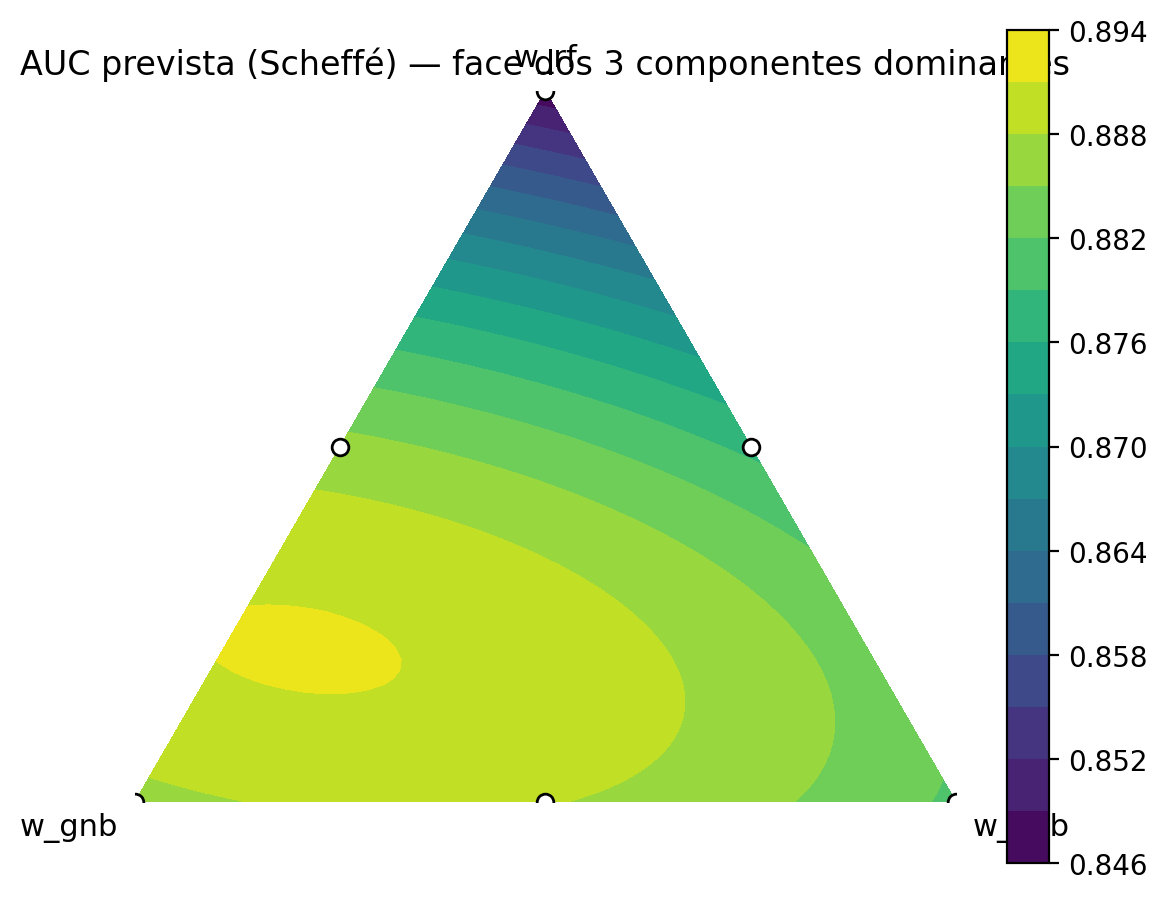
\includegraphics[width=0.9\columnwidth]{Figures/fig3_ternary_auc.png}}
\caption{Superfície de ROC-AUC prevista pelo metamodelo na face dos três componentes de maior peso (pontos brancos: corridas do arranjo nessa face).}
\label{fig:ternary}
\end{figure}

\begin{figure}[htbp]
\centerline{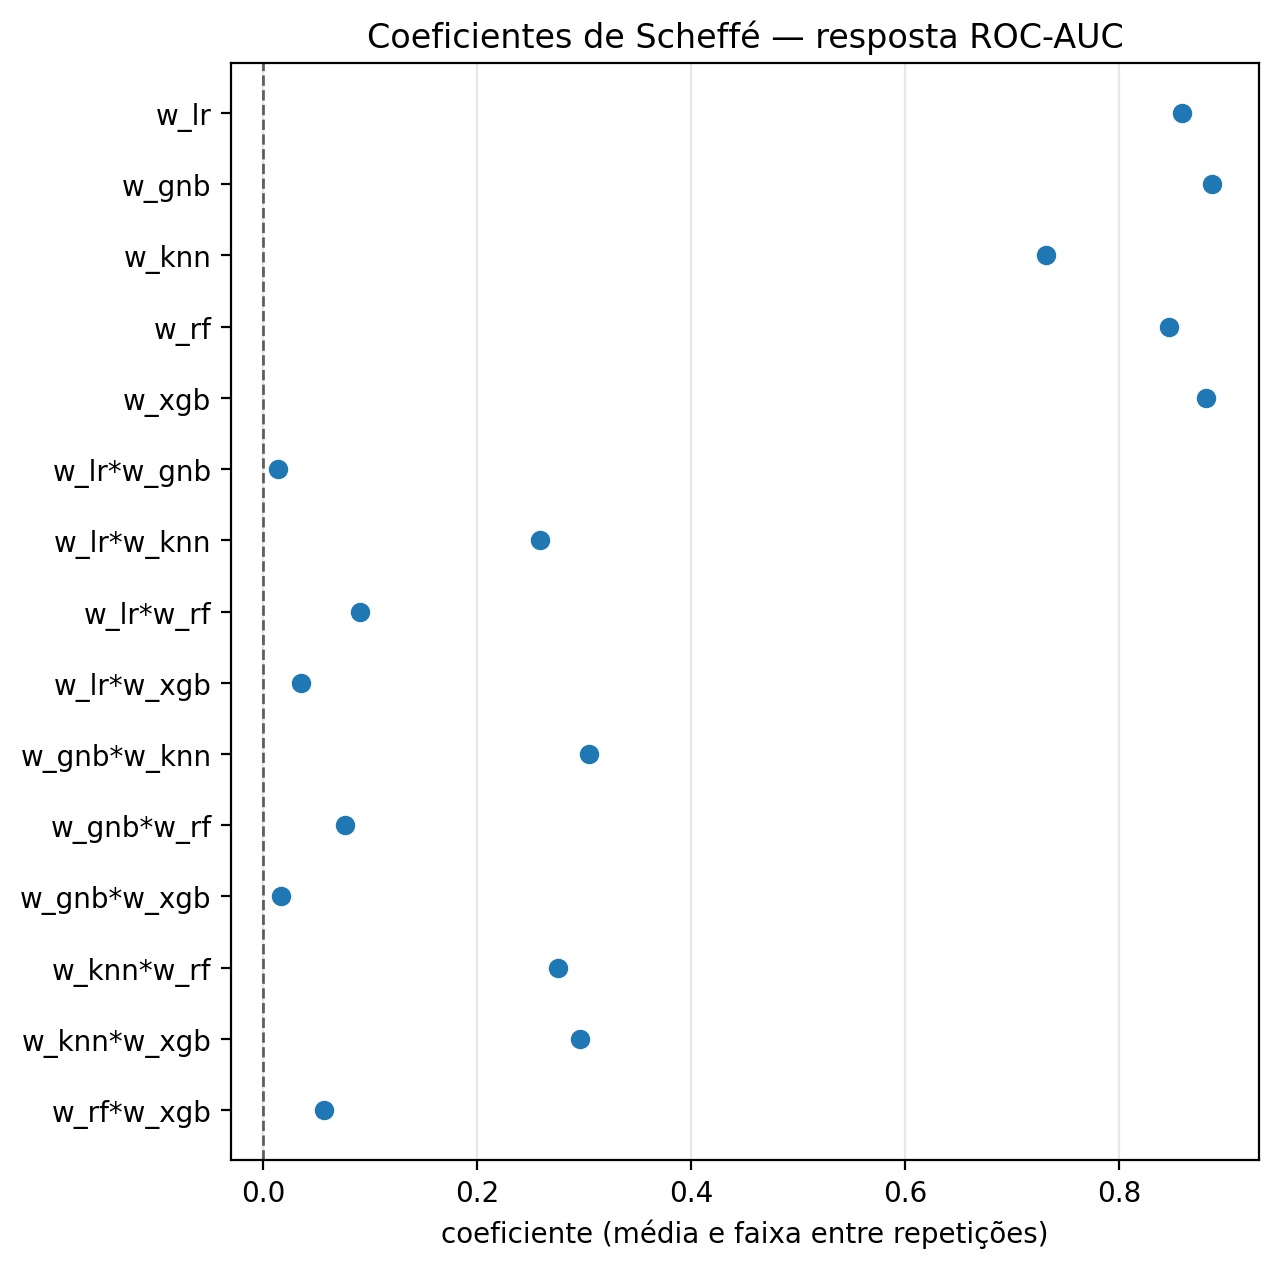
\includegraphics[width=\columnwidth]{Figures/fig4_scheffe_coefficients.png}}
\caption{Coeficientes do polinômio de Scheffé para a resposta ROC-AUC: média e faixa (mín--máx) entre as duas repetições da validação cruzada.}
\label{fig:coef}
\end{figure}

\subsection{Comparação final no conjunto de teste}
A Tabela~\ref{tab:holdout} apresenta a confirmação única no holdout e a Fig.~\ref{fig:holdout} a visão gráfica. \HoldoutSummary\ O ótimo global direto de \eqref{eq:opt} concentrou-se em dois componentes — 67\% Naive Bayes e 33\% XGBoost —, e o ótimo do metamodelo concordou nos componentes dominantes, com diferença de perda logarítmica OOF de \GapMetaDirect\ (cerca de 6\% da amplitude da superfície): a direção Naive Bayes--$k$-NN é quase plana perto do ótimo, e o metamodelo distribui ali um peso que a otimização direta não distribui. Nos testes $t$ corrigidos \eqref{eq:nb} sobre as 10 rodadas OOF, \StatsSummary

\begin{table}[htbp]
\caption{Confirmação no holdout (20\%; limiar de F1 escolhido na OOF)}
\begin{center}
\scriptsize\setlength{\tabcolsep}{3.5pt}
\begin{tabular}{lccccc}
\toprule
Método & ROC-AUC & log-loss & Brier & F1 & Ac.\ bal. \\
\midrule
Melhor modelo individual & 0{,}8822 & 0{,}2170 & 0{,}0624 & 0{,}536 & 0{,}753 \\
Voto uniforme ($w_j{=}1/5$) & 0{,}8896 & 0{,}2271 & 0{,}0663 & 0{,}547 & 0{,}755 \\
Stacking (reg.\ logística) & 0{,}8863 & 0{,}2171 & 0{,}0615 & 0{,}549 & 0{,}758 \\
SLSQP direto (log-loss) & 0{,}8890 & 0{,}2115 & 0{,}0608 & 0{,}549 & 0{,}763 \\
Mistura Scheffé (log-loss) & 0{,}8849 & 0{,}2154 & 0{,}0620 & 0{,}541 & 0{,}755 \\
Mistura Scheffé (AUC) & 0{,}8861 & 0{,}2190 & 0{,}0634 & 0{,}543 & 0{,}756 \\
\bottomrule
\end{tabular}
\label{tab:holdout}
\end{center}
\end{table}

\begin{figure}[htbp]
\centerline{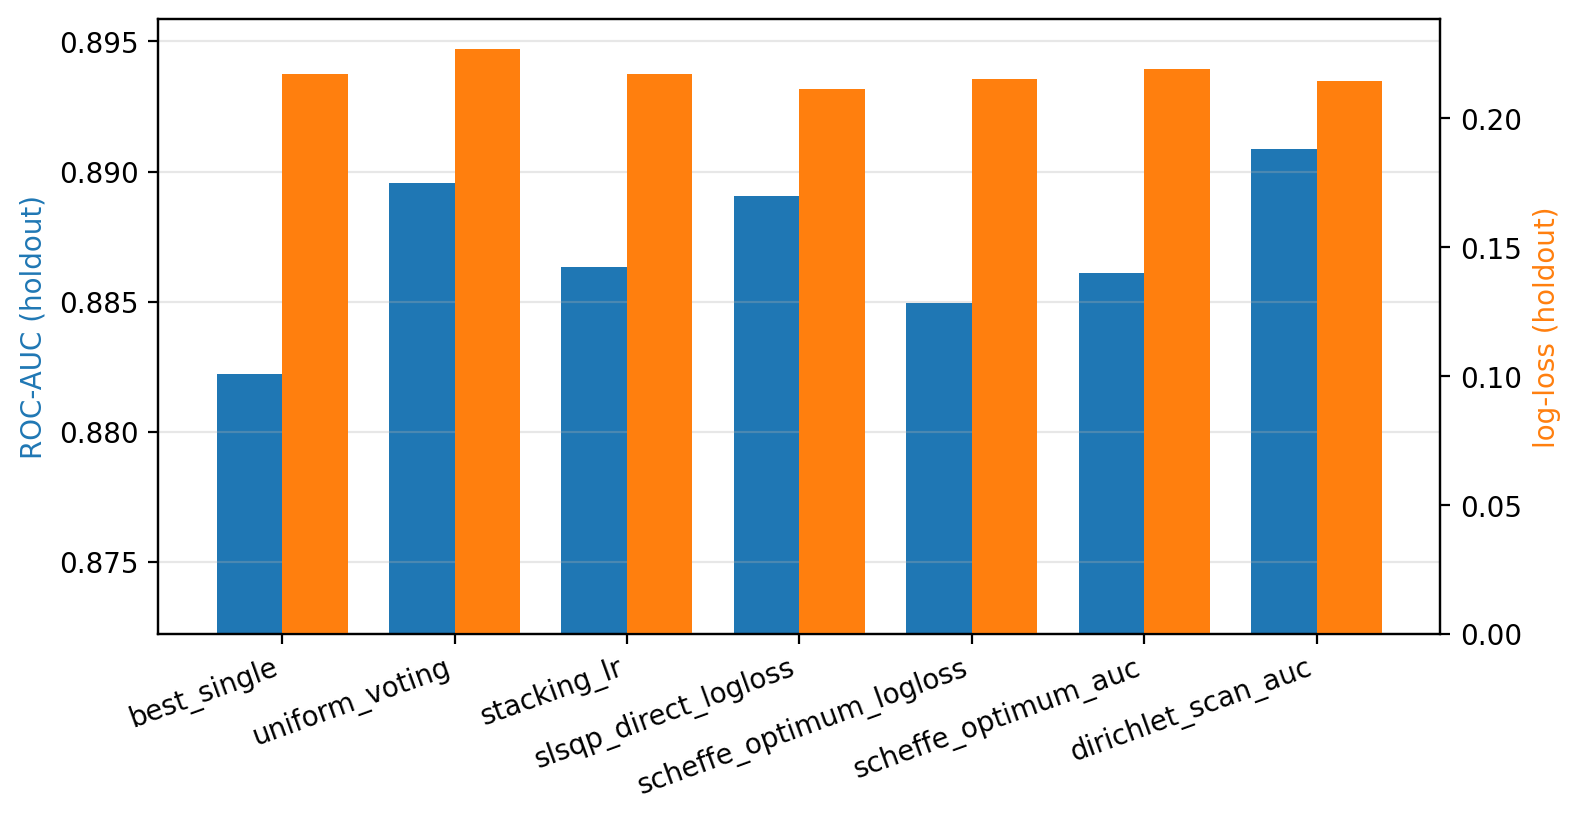
\includegraphics[width=\columnwidth]{Figures/fig5_holdout_comparison.png}}
\caption{ROC-AUC e perda logarítmica no holdout por método.}
\label{fig:holdout}
\end{figure}

A divergência esperada entre os pesos ótimos sob AUC e sob perda logarítmica materializou-se de forma mais branda que o antecipado: o Naive Bayes permaneceu dominante nas duas métricas (peso \NBWeightAUC\ sob AUC e \NBWeightLL\ sob perda logarítmica no ótimo do metamodelo), pois o recorte de probabilidades em $\varepsilon=10^{-3}$ domestica sua superconfiança; a diferença aparece na distribuição do peso restante, que sob AUC se espalha também por XGBoost e Random Forest. O custo computacional total do estudo foi de \TotalWallMin\ minutos em um laptop (Apple M4 Max), dominado pelos ajustes do Random Forest; a avaliação dos 46 pontos de pesos custou segundos, por operar sobre as matrizes OOF.

\section{Discussão}
\textbf{Interpretação.} A leitura conjunta dos coeficientes responde à pergunta de pesquisa: a superfície de desempenho é suave, côncava na direção das misturas e com região quase ótima ampla no interior do simplex — o que explica mecanicamente por que o voto uniforme é um \emph{baseline} difícil de superar e por que os ganhos da otimização de pesos, embora reais, são moderados. Os termos cruzados dominantes identificam os pares de famílias que efetivamente se complementam, informação que a seleção gulosa \cite{b4} e o stacking \cite{b2} não expõem.

\textbf{Comparação com stacking.} O stacking logístico, com pesos livres e intercepto, tem capacidade estritamente maior que a combinação convexa — e ainda assim não a superou: a mistura restrita ao simplex obteve perda logarítmica menor no holdout e OOF ($t$ corrigido significativo), evidência de que a restrição de não negatividade com soma unitária atua como regularização eficaz, em linha com a observação clássica de Breiman \cite{b3}, com a vantagem adicional de pesos legíveis como proporções.

\textbf{Limitações.} O estudo usa um único conjunto de dados, com variáveis anonimizadas (EDA apenas estrutural); as faixas de estabilidade dos coeficientes derivam de apenas duas repetições da validação cruzada e medem robustez à repartição, não incerteza amostral plena; o teste $t$ corrigido é aproximado com um único conjunto; os resultados no holdout interno não são comparáveis ao \emph{leaderboard} da competição (o conjunto de teste oficial não tem rótulos e contém linhas sintéticas); e as configurações fixas, sem ajuste de hiperparâmetros, limitam o teto de desempenho absoluto — decisão deliberada para manter o foco na metodologia de combinação, não no ajuste fino.

\section{Conclusão e Trabalhos Futuros}
Este trabalho formulou a ponderação de ensembles como um experimento com misturas e demonstrou, em um conjunto real de competição, que (i) o polinômio de Scheffé ajustado sobre um arranjo de \DesignRuns\ corridas resume fielmente a superfície de perda logarítmica (validação externa com erro de \RelRmseLL\ da amplitude e $R^2$ externo de 0,95), (ii) a mistura otimizada supera o melhor modelo individual, o stacking e o voto uniforme em perda logarítmica no teste — com o ótimo do metamodelo concordando com o ótimo global direto nos componentes dominantes — e é estatisticamente indistinguível do voto uniforme em ROC-AUC, resultado que a própria superfície explica (região quase ótima ampla contendo o centroide), e (iii) os coeficientes fornecem uma leitura interpretável de contribuições e complementaridades entre famílias de modelos, com o par Naive Bayes--XGBoost dominando a mistura ótima. Como trabalhos futuros propõem-se: a replicação do protocolo em outros regimes de dados (BNP Paribas Cardif, com perda logarítmica oficial e forte presença de faltantes; Porto Seguro, com desbalanceamento severo), a extensão multiobjetivo (desempenho \emph{versus} custo de inferência, linear nos pesos) com fronteiras de Pareto via NBI, e o estudo do comportamento do metamodelo sob componentes deliberadamente redundantes.

\begin{thebibliography}{00}
\bibitem{b1} T. G. Dietterich, ``Ensemble methods in machine learning,'' in \emph{Multiple Classifier Systems}, LNCS 1857, Springer, 2000, pp. 1--15.
\bibitem{b2} D. H. Wolpert, ``Stacked generalization,'' \emph{Neural Networks}, vol. 5, no. 2, pp. 241--259, 1992.
\bibitem{b3} L. Breiman, ``Stacked regressions,'' \emph{Machine Learning}, vol. 24, pp. 49--64, 1996.
\bibitem{b4} R. Caruana, A. Niculescu-Mizil, G. Crew, and A. Ksikes, ``Ensemble selection from libraries of models,'' in \emph{Proc. 21st Int. Conf. Machine Learning (ICML)}, 2004, pp. 137--144.
\bibitem{b5} A. Krogh and J. Vedelsby, ``Neural network ensembles, cross validation, and active learning,'' in \emph{Advances in Neural Information Processing Systems 7}, 1995, pp. 231--238.
\bibitem{b6} H. Scheffé, ``Experiments with mixtures,'' \emph{J. Royal Statistical Society B}, vol. 20, no. 2, pp. 344--360, 1958.
\bibitem{b7} J. A. Cornell, \emph{Experiments with Mixtures: Designs, Models, and the Analysis of Mixture Data}, 3rd ed. New York: Wiley, 2002.
\bibitem{b8} T. Chen and C. Guestrin, ``XGBoost: a scalable tree boosting system,'' in \emph{Proc. 22nd ACM SIGKDD}, 2016, pp. 785--794.
\bibitem{b9} L. Breiman, ``Random forests,'' \emph{Machine Learning}, vol. 45, pp. 5--32, 2001.
\bibitem{b10} C. Nadeau and Y. Bengio, ``Inference for the generalization error,'' \emph{Machine Learning}, vol. 52, pp. 239--281, 2003.
\bibitem{b11} R. R. Bouckaert and E. Frank, ``Evaluating the replicability of significance tests for comparing learning algorithms,'' in \emph{Proc. PAKDD}, 2004, pp. 3--12.
\bibitem{b12} F. Pedregosa \emph{et al.}, ``Scikit-learn: machine learning in Python,'' \emph{J. Machine Learning Research}, vol. 12, pp. 2825--2830, 2011.
\bibitem{b13} Kaggle, ``Santander Customer Transaction Prediction,'' 2019. [Online]. Disponível: https://www.kaggle.com/competitions/santander-customer-transaction-prediction
\bibitem{b14} C. Deotte, ``Modified naive Bayes --- Santander --- 0.899,'' Kaggle Notebook, 2019. [Online]. Disponível: https://www.kaggle.com/code/cdeotte/modified-naive-bayes-santander-0-899
\end{thebibliography}

\end{document}
